\documentclass{article}

\usepackage{graphicx}

\author{Nic Hollingum - 308193415}
\title{Computational Geometry - Assignment 4}

\addtolength{\oddsidemargin}{-.875in}
\addtolength{\evensidemargin}{-.875in}
\addtolength{\textwidth}{1.75in}
\addtolength{\topmargin}{-1in}
\addtolength{\textheight}{2.5in}

\begin{document}
\maketitle

\section {Euclidian Problems}

\subsection*{a}
By the triangle inequality, this is trivial, we shall prove it by contradiction.
We have a cycle of nodes which we vist, and removing nodes from the cycle represents removing elements to form a subset.
Conversely adding nodes represents increasing a subset to the size of the set.
In order for a subset not to be shorter than the superset, then there must exist some superset shorter than its subset.
In other words we have to decrease the length of the cycle by adding a node, or, we stop at some node in the cycle, move to the new node, then back to the next node in the cycle and continue.
But this requires the sum of paths from some node in the cycle to new node, and new node back to next, be less than some node to the next, which violates the triangle inequality (if a, b and c are edges of a triangle, then the length of any 1 must be less than the sum of the other 2).

\subsection*{b}
Proof by example:

\begin{figure}[htb]
\begin{center}
\leavevmode
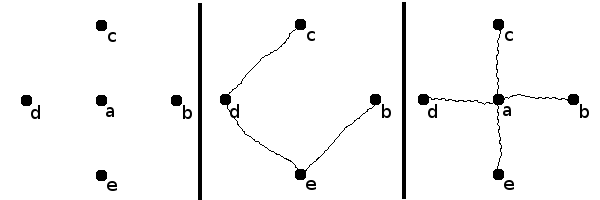
\includegraphics[width=0.6\textwidth]{mst.png}
\end{center}
\label{fig:mst}
\end{figure}

Using the 5 points here, where our subset lacks point ``a'', we see that the MST grows longer.
When a is absent, we must choose 3 of the 6 edges in $k_4$, and the 3 shortest edges are those around the perimeter.
Each of the perimeter points is 1 unit up, down, left or right of a, and the border edges have length $\sqrt 2$ accordingly, the total length is $3 \sqrt 2 = 4.24$.
When a is present then the MST is 4 edges from a to all of the corner points.
Each corner point is 1 unit distance from A, and so the MST has length 4, which is less than above.
Therefore even though the middle graph is a subset of the left, it has a longer MST than the right.

\subsection*{c}
First TSP must be more than MST, this can be verified by a counting problem, and that MST is a tree and TSP is a cycle.
given n points, where each is equidistant from evey other (we need n-1 dimensions to do this by the way) we note that the MST must have n-1 edges and so n-1 length, but the cycle must return to its start node, and so must have n edges and n length.
If the points are not equidistant we know that if the TSP is able to choose a shorter path, the MST is as well, but there are times when the MST can avoid long paths where the TSP cant.
Consider many points spread out evenly along a circle edge, with a gap on one side.
The MST is able to avoid this gap and simply choose the points around the perimeter, wheres at TSP will either take this edge, or backtrack along other edges and so waste time.

We also note that given an MST, we are able to find some repeating cycle, using depth-first search along all branches of the tree.
The salesman starts at some node in the tree and traverses it depth first.
Each edge must be crossed once to go to new nodes, and again later to return prom them, hence exactly twice.
Therefore we have a repeating cycle no more than double the length of the MST which visits every node.
Clearly a more efficient TSP can be contrived by skipping nodes we know we have visited and we will return from.
Such that if we would return from a to b, then b to it's parent c, we simply go from a to c and save the distance, therefore optimal TSP must be less or equal to 2*MST.

\section {Voronoi Convex Hull}

\section {MST and Delauny}

\section {Interval Range Query}

\section {t-Spanner}

\begin{thebibliography}{9}

\bibitem{tb}
	Mark de Berg and Otfried Cheong and Marc van Kreveld and Mark Overmar,
	\emph{Computational Geometry, Algorithms and Applications}.
	\emph{3rd ed, pp184-185}.
	Springer-Verlag Berlin Heidelberg
\end{thebibliography}

\end{document}
